\section{\texorpdfstring{Course Syllabus
}{Course Syllabus }}\label{course-syllabus}

\begin{longtable}[]{@{}
  >{\raggedright\arraybackslash}p{(\columnwidth - 2\tabcolsep) * \real{0.2727}}
  >{\raggedright\arraybackslash}p{(\columnwidth - 2\tabcolsep) * \real{0.7273}}@{}}
\toprule\noalign{}
\begin{minipage}[b]{\linewidth}\raggedright
Course Name
\end{minipage} & \begin{minipage}[b]{\linewidth}\raggedright
Organic Chemistry 2 (Laboratory)
\end{minipage} \\
\midrule\noalign{}
\endhead
\bottomrule\noalign{}
\endlastfoot
Semester & AY 23--24 Spring \\
Units & 2 \\
Department & Chemistry and Biochemistry \\
Time & TR 9:00--11:50 pm
(\hyperref[note-about-the-duration-of-a-lab-session]{see note below}) \\
Location & Science 1-350 \\
Instructor & Dr.~Hubert Muchalski \\
Coordinator & Dr.~Hubert Muchalski \\
Email & hmuchalski@mail.fresnostate.edu \\
Office phone & 559-278-2711 \\
Office & Science 1, room 352 \\
Office hours & Monday 15:00-15:50 and by
\href{https://calendar.app.google/mUmzNPCnZLXESrCQ8}{appointment} \\
\end{longtable}

\subsection{\texorpdfstring{Note about the duration of a lab session
}{Note about the duration of a lab session }}\label{note-about-the-duration-of-a-lab-session}

The CSU defines \emph{one class hour} as 50 minutes of instruction,
which is the default duration for a 1-unit lecture. Science laboratories
fall under the category of \emph{supervision courses}
(\href{https://academics.fresnostate.edu/scheduling/documents/CourseClassificationSystem%201.3.18.pdf}{C16
category}). For laboratory sessions, 1 unit corresponds to \emph{3 class
hours}, totaling 150 minutes (2 hours and 30 minutes) of
instruction/supervision. This differs from the duration listed in the
catalog (2 hours and 50 minutes) because it includes a 10-minute break
after each 50 minutes of instruction. However, adhering to fixed time
frame in a lab setting is challenging because work is
asynchronous---students work at their own pace, often in groups. Having
fixed times for breaks might be impractical or unsafe. Consequently, on
days when we work without a break, our goal will be to finish the lab
session by 11:30 (3:30 for PM sections), after 150 minutes of
instruction/supervision.

\subsection{\texorpdfstring{How to use this syllabus
}{How to use this syllabus }}\label{how-to-use-this-syllabus}

This document contains all the information you need to navigate the
course. \emph{Read it once giving it your full attention}, then search
as needed. Use the table of contents found in the sidebar of the web
version or use \texttt{Ctrl/Cmd+F} to bring up a search field, and then
type in the text you are looking for.

\begin{itemize}
\tightlist
\item
  When you see blue- or purple-underlined text in the syllabus or any
  other document, it's a clickable link. For example,
  \href{https://start.duckduckgo.com/?q=dogs+wearing+clothes&iar=images&iax=images&ia=images&kp=1}{click
  here for pictures of dogs in clothes}.
\item
  Links to all important documents and information can be found on the
  course \href{https://fresnostate.instructure.com/courses/76128}{Canvas
  site}
\item
  Once the syllabus is finalized, it will be available in electronic
  form (here) and as a PDF on Canvas. After that, the electronic version
  will be updated as needed.
\end{itemize}

\subsection{\texorpdfstring{Table of Contents
}{Table of Contents }}\label{table-of-contents}

\begin{itemize}
\tightlist
\item
  \hyperref[about-the-course]{About the course}

  \begin{itemize}
  \tightlist
  \item
    \hyperref[assumed-prior-knowledge-and-skills]{Assumed prior
    knowledge and skills}
  \end{itemize}
\item
  \hyperref[course-learning-outcomes]{Course Learning Outcomes}
\item
  \hyperref[course-materials-and-technology]{Course materials and
  technology}
\item
  \hyperref[course-workflow]{Course workflow}
\item
  \hyperref[on-keeping-records-lab-notebook]{On keeping records (lab
  notebook)}

  \begin{itemize}
  \tightlist
  \item
    \hyperref[lab-notes-guiding-principles]{Lab notes guiding
    principles}
  \end{itemize}
\item
  \hyperref[assessments-and-grading]{Assessments and grading}

  \begin{itemize}
  \tightlist
  \item
    \hyperref[grading-philosophy]{Grading philosophy}
  \item
    \hyperref[grading-of-experiments]{Grading of experiments}
  \item
    \hyperref[research-project]{Research project}
  \item
    \hyperref[letter-grades]{Letter grades}
  \end{itemize}
\item
  \hyperref[safe-chemical-laboratory-practices]{Safe Chemical Laboratory
  Practices}
\item
  \hyperref[policies-and-disclaimers]{Policies and disclaimers}

  \begin{itemize}
  \tightlist
  \item
    \hyperref[attendance-and-make-up-policy]{Attendance and make-up
    policy}
  \item
    \hyperref[technology-issues-when-submitting-work]{Technology issues
    when submitting work}
  \item
    \hyperref[academic-dishonesty]{Academic Dishonesty}
  \item
    \hyperref[dropping-the-course-after-the-census-date]{Dropping the
    course after the census date}
  \item
    \hyperref[plagiarism-detection]{Plagiarism detection}
  \item
    \hyperref[intellectual-property]{Intellectual Property}
  \item
    \hyperref[dispute-resolution]{Dispute Resolution}
  \item
    \hyperref[student-ratings-of-instruction]{Student Ratings of
    Instruction}
  \end{itemize}
\item
  \hyperref[university-policies-and-disclaimers]{University policies and
  disclaimers}

  \begin{itemize}
  \tightlist
  \item
    \hyperref[links-to-relevant-university-policies]{Links to relevant
    University Policies}
  \end{itemize}
\item
  \hyperref[university-services]{University Services}
\item
  \hyperref[course-calendar]{Course Calendar}
\item
  \hyperref[appendix-a-rubrics]{Appendix A: Rubrics}

  \begin{itemize}
  \tightlist
  \item
    \hyperref[lab-readiness]{Lab readiness}
  \item
    \hyperref[risk-assessment-rubric]{Risk assessment rubric}
  \item
    \hyperref[lab-notebook-rubric]{Lab notebook rubric}
  \item
    \hyperref[experimental-results-rubric]{Experimental results rubric}
  \item
    \hyperref[grading-of-lab-reports-and-the-emrn-rubric]{Grading of lab
    reports and the EMRN rubric}
  \item
    \hyperref[research-report-and-presentation]{Research report and
    presentation}
  \end{itemize}
\end{itemize}

\subsection{About the course}\label{about-the-course}

The aim of this course is to inspire students to explore the breadth of
organic chemistry, fostering an understanding of its principles and
their practical application. This, in turn, equips students with a
functional knowledge and genuine appreciation of organic structure and
reactivity. In the second semester of the sequence, the emphasis shifts
towards the pivotal role of experimentation in gaining molecular
insights. This involves correlating molecular structure, reactivity, and
function through the use of wet chemical methods and spectroscopy.

CHEM 129B is the second part of the 2-semester sequence in organic
chemistry laboratory. As such it is primarily concerned with introducing
intermediate level concepts and techniques used in organic chemistry. We
will continue to use the techniques covered in the first semester lab
and will introduce additional methods and techniques such as NMR
spectroscopy, multi-step synthesis, green chemistry, and chemical
literature.

\subsubsection{Assumed prior knowledge and
skills}\label{assumed-prior-knowledge-and-skills}

The formal pre-requisite to enroll in CHEM 129B is passing CHEM 129A (or
equivalent) with a grade of ``C'' or better. In practice it means that
students who enroll in CHEM 129B should be able to:

\begin{itemize}
\tightlist
\item
  communicate the structure and properties of organic molecules using
  common drawing and naming conventions;
\item
  conduct laboratory work of high quality including handling chemicals
  and other laboratory hazards in a safe, ethical, and socially
  responsible manner;
\item
  use basic laboratory techniques such as extraction, crystallization,
  filtration, distillation, column chromatography, TLC; and
\item
  measure melting point and acquire IR spectrum of a sample.
\end{itemize}

\subsection{Course Learning Outcomes}\label{course-learning-outcomes}

Upon completion of this course, students will be able to:

\begin{itemize}
\tightlist
\item
  Keep accurate, clear, concise, and complete records of their
  laboratory work in a notebook that would allow a trained organic
  chemist to reproduce the results.
\item
  Describe what you see (macroscopic) with chemical language
  (microscopic \& sub-microscopic).
\item
  Design ways you can separate a mixture into its components by
  manipulating physical and chemical properties.
\item
  Use standard laboratory equipment and instruments and evaluate the
  reliability and significance of laboratory data, all within
  professional ethical guidelines.
\item
  Use online databases to find relevant research articles containing
  information such as physical and chemical properties of organic
  molecules, synthetic procedures, and spectroscopic data.
\item
  Rationalize physical phenomena using polarity and intermolecular
  forces.
\item
  Plan a synthesis experiment by evaluating the information found in
  online databases and research articles.
\item
  Carry out an experimental procedure to synthesize, isolate, purify,
  and analyze the product of chemical synthesis.
\item
  Analyze the results of an experiment and be able to identify sources
  of error and suggest improvements.
\item
  Interpret spectroscopic data of organic compounds to confirm the
  structure of organic compounds.
\item
  Communicate the results of experiments to the instructor and peers in
  written form (lab report) and presentation (slide deck or poster).
\end{itemize}

For more details refer to \href{/a5Vq_rZQRI2_f6ylivvNiA}{Department
Student Learning Outcomes} modeled after
\href{https://www.acs.org/education/policies/acs-approval-program/guidelines.html}{ACS
Guidelines for Bachelor's Degree Programs}.

\subsection{Course materials and
technology}\label{course-materials-and-technology}

\begin{itemize}
\tightlist
\item
  \textbf{Techniques Reference Manual}
  \href{https://chem.libretexts.org/Bookshelves/Organic_Chemistry/Book:_Organic_Chemistry_Lab_Techniques_(Nichols)}{LibreTexts
  e-book by Lisa Nichols} is our recommended reference for laboratory
  techniques. The textbook by Pavia et al.~is listed as the official
  textbook for this course, but we are in the process of phasing it out.
  If you own a copy of Pavia's textbook (5th or 6th edition), then feel
  free to use it in addition to the LibreTexts option
\item
  \textbf{Personal protective equipment (PPE)}: Lab coat and approved
  safety goggles. Disposable nitrile gloves will be provided.
\item
  \textbf{Canvas:} The central repository for all course materials and
  information is our
  \href{https://fresnostate.instructure.com/courses/76128}{Canvas site}
  which will be the main repository for assignments, grades, and links
  to materials/resources.
\item
  \textbf{Document scanning tool}: Most documents you will turn in for
  feedback and grading will be submitted electronically but prepared on
  paper. A smartphone with a scanning app can be used to convert paper
  documents into PDFs. There are number of free options available for
  both iOS and Android. Find one that you like and learn how to use it.
\item
  \textbf{Personal computer:} You will need a x86 class personal
  computer\footnote{Chromebooks and iPads are a powerful devices but are
    not x86-class computers. They can't run ChemDraw or MestReNova
    software (at least not yet).} that can run standalone desktop
  applications. Mobile devices can be used but they are inferior or
  incompatible with software we will use.
\end{itemize}

\subsection{Course workflow}\label{course-workflow}

Activities in this course follows a cyclical pattern. Over the semester
you will engage in 5 experimental modules and an independent research
project. At the heart of each module is a synthesis of an organic
compound (1--3 steps). Specific requirements will be communicated by the
instructor at the beginning of the semester.

\textbf{Before class}, your task will be to prepare for the experiment
by studying the relevant reactions and mechanisms, lab techniques, and
safety information about chemicals you will be work-ing with. Your
instructor may assign graded pre-lab assignment to help you prepare for
the lab.

\textbf{Class time} will be focused primarily on doing experiments,
making observations, generating results, processing spectroscopic data,
and group discussions. Results and observations made during lab are
important inputs for writing post-lab reports. For example, not making a
key observation or obtaining poor quality data may reduce your grade on
the experiment because you will not have all information to write the
lab report or discuss the results.

\textbf{After class} you will work on finalizing the documentation
related to the experiment, usually in a form of typed lab report.
Details for each post-lab assignment will be posted on Can-vas by the
instructor. Document templates will be available for formal lab reports.

\subsection{On keeping records (lab
notebook)}\label{on-keeping-records-lab-notebook}

The human brain is both the least reliable whiteboard and the least
dependable alarm clock. It's crucial to acknowledge that memories of
your actions and observations in the lab can fade rapidly once you step
away. To counteract this, it's essential to document your experiences in
real time, as these notes (combined with pre-lab documentation) will
serve as the foundation for your subsequent post-lab tasks, such as
reports and presentations.

Maintain a comprehensive record of what you did and observed. Also keep
all physical copies such as IR and NMR spectra, gas chromatograms, and
sketches of TLC plates. These components contribute to your experimental
record. Remember that your lab notes are subject to evaluation at any
point and should remain up-to-date. Your instructor will provide
guidelines on how to maintain your laboratory notebook at the start of
the semester. Be prepared to submit your in-lab notes for assessment
before concluding your time in the lab. your time in the lab.

\subsubsection{Lab notes guiding
principles}\label{lab-notes-guiding-principles}

Lab notes should document what you did and how, what you observed, and
the data you collected. To know what to write and not to write in the
notebook is a balancing act of relevance and brevity. You need write
down details that are relevant and necessary for someone to reproduce
your work. This hypothetical chemist will not be able to consult with
you or have access to any auxiliary documentation that you had access to
while doing the experiment. Therefore, you need to describe what you did
and how.

It is safe to assume, however, that the reader of your notes has been
trained in the basic organic laboratory techniques. For example, you
don't have to explain how to do a recrystallization because the reader
who will should know how to carry out recrystallization (and if not,
they can refer to a techniques manual). What will be helpful to them are
the details relevant to this particular recrystallization: solvent used,
approximate volume of solvent, time it took to cool and grow crystals.

Lab notes should be easy to read---use paragraph breaks, headings, etc.
to help the reader navigate the notebook.

Contrary to common belief, reproducible and detailed lab notes don't
have to be long and take a lot of time and effort to produce. Below is
an example statement that captures all important information about
purification of the crude material, yield, and the appearance of the
final product:

\begin{quote}
``The crude product (sticky brown solid, 1.23 g) was recrystallized from
hot ethanol (15 mL) in an Erlenmeyer flask. After cooling to rt and then
to 0 °C, the solid was collected by vacuum filtration, washed with
ice-cold water, and dried in air for 1 h to give the product as a white
crystalline solid (0.38 g), mp 87--89 °C.''
\end{quote}

Additional benefit of writing it all down in real time is that it can
help you track down errors, explain unexpected outcomes, and/or
troubleshoot the experiment that went wrong. In the recrystallization
described above, the mass recovery is quite poor and a chemist repeating
the experiment may decide to use less ethanol (or a different solvent)
to improve the mass recovery.

\subsection{Assessments and grading}\label{assessments-and-grading}

The final grade in the course will be based on your work in three areas
(see table below). There will be four experiment sets, independent
project, and quizzes. Each experiment set will have variety of graded
work (pre-lab, lab notebook, report, and other assignments) that add
contributes to the 15\% value for each lab set.

\begin{longtable}[]{@{}ll@{}}
\toprule\noalign{}
Assignment Category & \%Weight \\
\midrule\noalign{}
\endhead
\bottomrule\noalign{}
\endlastfoot
Experiments (4×15) & 60\% \\
Research Project & 30\% \\
Quizzes & 10\% \\
\textbf{Total} & \textbf{100\%} \\
\end{longtable}

\subsubsection{Grading philosophy}\label{grading-philosophy}

Grading in this course is different than you might be used to. Please
read this section carefully and ask questions as needed.

As a teacher and learner, I strongly believe that \emph{learning takes
time} and that grading your work based on a single point of data, such
as a single quiz or test, is inaccurate, invalid, and perhaps unethical.
A truly valid measure of learning has to involve \emph{multiple
attempts} that allow you to learn from your past mistakes and
demonstrate not only your skill, but also your growth. I believe your
work should be evaluated by just like everyone else's work in the real
world is evaluated, i.e., by giving you \emph{clearly defined standards}
for quality, \emph{detailed verbal feedback} on your work, and
\emph{opportunities to try again} based on the feedback. This gets you
into a \emph{feedback loop}, a conversation between you and me about
your work, that continues until your work meets the standards (or we
reach the end of the semester). In light of the principles outlined
above, in this course students can \emph{revise and resubmit some of
their work}, several times over if needed, using the feedback at each
stage to improve and grow.

\subsubsection{Grading of experiments}\label{grading-of-experiments}

You will receive feedback and marks on work that you produce in- and
outside the lab. Those include pre-lab documentation, experimental notes
and observations, results (yield, spectroscopic data), and written lab
report. Each of the regular experiments contributes 15\% to the final
grade and will have several components (see table below for details).

\begin{longtable}[]{@{}
  >{\raggedright\arraybackslash}p{(\columnwidth - 4\tabcolsep) * \real{0.5349}}
  >{\raggedright\arraybackslash}p{(\columnwidth - 4\tabcolsep) * \real{0.1163}}
  >{\raggedright\arraybackslash}p{(\columnwidth - 4\tabcolsep) * \real{0.3488}}@{}}
\toprule\noalign{}
\begin{minipage}[b]{\linewidth}\raggedright
Item
\end{minipage} & \begin{minipage}[b]{\linewidth}\raggedright
Value
\end{minipage} & \begin{minipage}[b]{\linewidth}\raggedright
Revision policy
\end{minipage} \\
\midrule\noalign{}
\endhead
\bottomrule\noalign{}
\endlastfoot
Pre-lab documentation & 2\% & Before the experiment begins \\
Risk assessment & 2\% & Before the experiment begins \\
In-lab notes & 3\% & No \\
Results & 3\% & No \\
Lab report & 5\% & Within one week after report returned with
comments \\
\end{longtable}

\subsubsection{Research project}\label{research-project}

During the second half of the semester, students will engage in an
independent research project known as a CURE (Course-based Undergraduate
Research Experience). The instructor will not provide the project's
objective and methods, and the outcomes are either entirely unknown or
only partially revealed. To accomplish the project, students will
conduct comprehensive literature research to gather the essential
information required for the synthesis. The culmination of this endeavor
will involve delivering a presentation to the class.

\subsubsection{Letter grades}\label{letter-grades}

Final grade will be determined based on overall performance according to
the weights in the table above.

\begin{longtable}[]{@{}ll@{}}
\toprule\noalign{}
Grade & Total Score \\
\midrule\noalign{}
\endhead
\bottomrule\noalign{}
\endlastfoot
A & 90--100\% \\
B & 80--89\% \\
C & 70--79\% \\
D & 60-69\% \\
F & \textless60\% \\
\end{longtable}

\subsection{Safe Chemical Laboratory
Practices}\label{safe-chemical-laboratory-practices}

\begin{enumerate}
\def\labelenumi{\arabic{enumi}.}
\tightlist
\item
  NO food or drink in the laboratory.
\item
  Wear clothing appropriate for laboratory work.
\item
  Select and correctly use appropriate Personal Protective Equipment
  (PPE).
\item
  Know what to do and who to contact in an emergency in the laboratory.
\item
  Avoid distractions and be alert to and aware of your surroundings and
  potential hazards in your area.
\item
  Maintain a safe and clean work area.
\item
  Only conduct experiments or procedures approved by your lab instructor
  or research advisor.
\item
  Understand the common chemical hazards and hazards specific to the
  chemicals and procedures with which you are working.
\item
  Understand and follow best practices on how to handle, transport,
  store, and dispose of chemicals safely.
\item
  If any equipment, glassware, or procedures are not working properly or
  as expected, notify your instructor before proceeding.
\item
  Notify your instructor if you have, develop, or may develop any
  medical conditions (e.g.~severe asthma, limited mobility, vision
  impairment, pregnancy, etc) that may affect your safety in the
  laboratory or sensitivity to chemicals, so that your instructor can
  properly advise or accommodate you on minimizing the risks associated
  with laboratory work.
\end{enumerate}

These principles will be discussed in detail during the first week of
class. More information can be found here: \url{https://goo.gl/1UFRbo}.
Also, refer to
\href{https://www.acs.org/content/dam/acsorg/about/governance/committees/chemicalsafety/publications/acs-safety-guidelines-academic.pdf}{\emph{Guidelines
for Chemical Laboratory Safety in Academic Institutions}} published by
American Chemical Society.

\subsection{Policies and disclaimers}\label{policies-and-disclaimers}

\subsubsection{Attendance and make-up
policy}\label{attendance-and-make-up-policy}

Students are expected to attend and actively participate in all class
sessions. If you are absent from class, it is your responsibility to
check on announcements made while you were away. The course attendance
policy follows university's
\href{http://www.fresnostate.edu/academics/facultyaffairs/documents/apm/232.pdf}{APM
232: Policy on Student Absence}. Late assignments will not be accepted
for a grade unless the absence meets the guidelines set forth by the
university policy. Excuses and exceptions will be interpreted will in
light of the APM 232.

\subsubsection{Technology issues when submitting
work}\label{technology-issues-when-submitting-work}

For assignments submitted electronically, it is your responsibility to
make sure they are submitted on time, through any means necessary, even
if technology issues arise. If a tech issue arises, it is your
responsibility to find another way to get it to the instructor (for
example, via an email attachment). Technology issues that are avoidable
or resolved with a simple work-around will not be considered valid
grounds for a deadline extension. For example, if you are trying to
upload a Lab to Canvas and Canvas won't accept the file, you should try
again later or send the file as an email attachment until you can upload
it successfully.

\subsubsection{Academic Dishonesty}\label{academic-dishonesty}

For most assignments you are allowed and encouraged to work with others.
However, the final product that you submit for feedback must be the
result of your own efforts. Therefore you may share ideas and strategies
with others, but collaboration on the actual finished product you submit
is not allowed. Your work is expected to be the product of your own
thinking, written and explained in your own words with no parts of the
work copied from external sources such as books or websites, and done
clearly enough in your own mind that you could explain the work from
start to finish if asked. Specifically, this excludes:

\begin{itemize}
\tightlist
\item
  copying work from another student;
\item
  copying work from a website;
\item
  copying work generated by an AI bot such as ChatGPT;
\item
  paraphrasing work done by another student or from print or Internet
  resources---i.e.,putting it in your own words---without coming up with
  the main ideas and strategies yourself; and
\item
  \emph{allowing or enabling} another student to copy or paraphrase work
  that you did, even if you did the original work yourself.
\end{itemize}

Violation of this policy is considered ``academic dishonesty'' and
carries with it strong punitive measures mandated by Fresno State,
including possible automatic failure of the course or suspension from
the university. For details, please see APM 235 by going to
\url{http://www.fresnostate.edu/aps/documents/apm/235.pdf}.

\subsubsection{Dropping the course after the census
date}\label{dropping-the-course-after-the-census-date}

A \emph{serious and compelling reason} is defined as an unexpected
condition that is not present prior to enrollment in the course that
unexpectedly arises and interferes with a student's ability to attend
class meetings and/or complete course requirements. The reason must be
acceptable to and verified by the instructor of record and the
department chair. The condition must be stated in writing on the
appropriate form. The student must provide documentation that
substantiates the condition.

Failing or performing poorly in a class is not an acceptable ``serious
and compelling reason'' within the University policy, nor is
dissatisfaction with the subject matter, class or instructor.

\subsubsection{Plagiarism detection}\label{plagiarism-detection}

The campus subscribes to Turnitin, a plagiarism prevention service,
through Canvas. You will need to submit written assignments to Turnitin.
Student work will be used for plagiarism detection and for no other
purpose. The student may indicate in writing to the instructor that
he/she refuses to participate in the plagiarism detection process, in
which case the instructor can use other electronic means to verify the
originality of their work. Turnitin Originality Reports WILL NOT be
available for your viewing.

\subsubsection{Intellectual Property}\label{intellectual-property}

All course materials, including but not limited to the syllabus,
readings, quiz questions, exam questions, and assignments prepared by
the instructor are property of the instructor and University. Students
are prohibited from posting course materials online (e.g., Course Hero)
and from selling course materials to or being paid for providing
materials to any person or commercial firm without the express written
permission of the professor teaching this course. Doing so will
constitute both an academic integrity violation and a copyright
violation. Audio and video recordings of class lectures are prohibited
unless I give you explicit permission in advance. Students with an
official letter from the Services for Students with Disabilities office
may record the class if SSD has approved that service. Otherwise,
recordings of lectures are included in the intellectual property notice
described above.

\subsubsection{Dispute Resolution}\label{dispute-resolution}

If there are questions or concerns that you have about this course that
you and I are not able to resolve, please feel free to contact the Chair
of the department to discuss the matter.

\begin{itemize}
\tightlist
\item
  Chair's name: Dr.~Krish Krishnan
\item
  Department name: Chemistry and Biochemistry
\item
  Chair's email: krish@csufresno.edu
\item
  Department phone number:
\end{itemize}

\subsubsection{Student Ratings of
Instruction}\label{student-ratings-of-instruction}

In the final weeks of the semester, you will be asked to complete a
short survey to provide feedback about this class. The primary goal of
student ratings is to help your instructor improve the class. Feedback
will also be reviewed by the department chair and the college dean. You
will be given 15 minutes of class time to complete student ratings.
Please offer feedback honestly and thoughtfully. Your participation is
appreciated. You can access your student rating surveys and get more
information at:
https://sites.google.com/mail.fresnostate.edu/fresno-state-sri/fssri-for-students.

\subsection{University policies and
disclaimers}\label{university-policies-and-disclaimers}

\subsubsection{Links to relevant University
Policies}\label{links-to-relevant-university-policies}

\begin{itemize}
\tightlist
\item
  Class Schedule Policies:
  \url{http://fresnostate.edu/studentaffairs/classschedule/policy/}
\item
  Copyright Policy: \url{http://libguides.csufresno.edu/copyright}
\item
  Students with Disabilities:
  \url{http://fresnostate.edu/studentaffairs/careers/students/interests/disabilities.html}
\item
  Academic Integrity and Honor Code:
  \url{http://www.fresnostate.edu/academics/facultyaffairs/documents/apm/236.pdf}
\item
  Policy on Cheating and Plagiarism:
  \url{http://fresnostate.edu/studentaffairs/studentconduct/policies/cheating-plagiarism.html}
\item
  Add/Drop Course:
  \url{http://www.fresnostate.edu/studentaffairs/registrar/registration/}
\item
  Computer requirements:
  \url{https://www.fresnostate.edu/catalog/academic-regulations/index.html#computerreq}
\item
  Disruptive classroom behavior:
  \url{http://www.fresnostate.edu/academics/facultyaffairs/documents/apm/419.pdf}
\end{itemize}

\subsection{University Services}\label{university-services}

\begin{itemize}
\tightlist
\item
  \href{http://fresnostateasi.org/}{Associated Students, Inc.}
\item
  \href{http://fresnostate.edu/studentaffairs/ssd/}{Students with
  Disabilities}
\item
  \href{http://fresnostate.edu/studentaffairs/dsc/index.html}{Dream
  Success Center}
\item
  \href{https://library.fresnostate.edu/}{Library}
\item
  \href{http://fresnostate.edu/studentaffairs/lrc}{Learning Center
  Information}
\item
  \href{https://www.fresnostate.edu/studentaffairs/health/}{Student
  Health and Counseling Center}
\item
  \href{https://studentaffairs.fresnostate.edu/lrc/supportnet/index.html}{SupportNet}
\item
  \href{https://studentaffairs.fresnostate.edu/survivoradvocate/}{Survivor
  Advocacy}
\item
  \href{http://www.fresnostate.edu/artshum/writingcenter/}{Writing
  Center}
\end{itemize}

\subsection{Course Calendar}\label{course-calendar}

This syllabus and schedule are subject to change in the event of
extenuating circumstances.

\begin{longtable}[]{@{}
  >{\raggedright\arraybackslash}p{(\columnwidth - 4\tabcolsep) * \real{0.0946}}
  >{\raggedright\arraybackslash}p{(\columnwidth - 4\tabcolsep) * \real{0.0946}}
  >{\raggedright\arraybackslash}p{(\columnwidth - 4\tabcolsep) * \real{0.8108}}@{}}
\toprule\noalign{}
\begin{minipage}[b]{\linewidth}\raggedright
Week of
\end{minipage} & \begin{minipage}[b]{\linewidth}\raggedright
Lab
\end{minipage} & \begin{minipage}[b]{\linewidth}\raggedright
Lab Activities
\end{minipage} \\
\midrule\noalign{}
\endhead
\bottomrule\noalign{}
\endlastfoot
15-Jan & Mon/Tue & NO LAB (MLK Holiday) \\
& Wed/Thu & NO LAB (Administrative Day) \\
22-Jan & Mon/Tue & Lab orientation, syllabus, chemical safety, locker
check-in. \\
& Wed/Thu & Module 1: Mechanochemistry (synthesis of chalcones) \\
29-Jan & Mon/Tue & Module 1: Mechanochemistry (synthesis of
chalcones) \\
& Wed/Thu & Module 1: Mechanochemistry (synthesis of chalcones) \\
5-Feb & Mon/Tue & Module 2: Renewable feedstocks and qNMR purity
assay \\
& Wed/Thu & Module 2: Renewable feedstocks and qNMR purity assay \\
12-Feb & Mon/Tue & Module 2: Renewable feedstocks and qNMR purity
assay \\
& Wed/Thu & Module 3: Synthesis with renewable feedstocks in water \\
19-Feb & Mon/Tue & NO LAB (President's Day) \\
& Wed/Thu & Module 3: Synthesis with renewable feedstocks in water \\
26-Feb & Mon/Tue & Module 3: Synthesis with renewable feedstocks in
water \\
& Wed/Thu & Module 3: Synthesis with renewable feedstocks in water \\
4-Mar & Mon/Tue & Module 4: Stereochemistry of Suzuki-Miyaura
reaction \\
& Wed/Thu & Module 4: Stereochemistry of Suzuki-Miyaura reaction \\
11-Mar & Mon/Tue & Module 4: Stereochemistry of Suzuki-Miyaura
reaction \\
& Wed/Thu & ACS NOLA ** Literature Research Tools (@Library) \\
18-Mar & Mon/Tue & Module 5: Research project \\
& Wed/Thu & Module 5: Research project \\
25-Mar & Mon/Tue & Spring Break Recess \\
& Wed/Thu & Spring Break Recess \\
1-Apr & Mon/Tue & NO LAB (Cesar Chavez) \\
& Wed/Thu & Module 5: Research project \\
8-Apr & Mon/Tue & Module 5: Research project \\
& Wed/Thu & Module 5: Research project \\
15-Apr & Mon/Tue & Module 5: Research project \\
& Wed/Thu & Module 5: Research project \\
22-Apr & Mon/Tue & Module 5: Research project \\
& Wed/Thu & Module 5: Research project \\
29-Apr & Mon/Tue & Module 5: Research project \\
& Wed/Thu & Module 5: Research project (clean-up \& wrap-up) \\
6-May & Mon/Tue & Module 5: Research project presentations \\
\end{longtable}

\subsection{Appendix A: Rubrics}\label{appendix-a-rubrics}

\subsubsection{Lab readiness}\label{lab-readiness}

\begin{itemize}
\tightlist
\item
  \textbf{Satisfactory (2)}: Prelab documentation (stoichiometry table,
  calculations, etc) is complete, accurate and conveys student's
  readiness to carry out the experiment.
\item
  \textbf{Progressing (1}): Prelab documentation (stoichiometry table,
  calculations, etc) is complete but contains errors or inaccuracies.
  The errors don't compromise student's readiness to carry out the
  experiment.
\item
  \textbf{Incomplete (0}): Prelab documentation was not submitted OR the
  submitted material is incomplete, contains critical errors or
  significant inaccuracies that compromise student's readiness for the
  experiment.
\end{itemize}

\subsubsection{Risk assessment rubric}\label{risk-assessment-rubric}

\begin{itemize}
\tightlist
\item
  \textbf{Complete (2)}: Hazard and risk assessment is complete,
  accurate, and relevant to the experiment. Significant risks and
  hazards are identified and a safety recommendation is provided. Errors
  are insignificant or inconsequential
\item
  \textbf{Progressing (1)}: Hazard and risk assessment is provided but
  significant gaps remain, the safety information is inaccurate or not
  irrelevant to the experiment.
\item
  \textbf{Incomplete (0)}: Safety information is not provided OR the
  information provided significantly increases the risk of exposure to
  hazards.
\end{itemize}

\subsubsection{Lab notebook rubric}\label{lab-notebook-rubric}

The notes will allow others to reproduce the work. The notes include
observations and communicate what was done, how, when, and by whom.

\begin{itemize}
\tightlist
\item
  \textbf{Fully reproducible (3)}: The notes are complete and include
  all key information. A person unfamiliar with the experiment is highly
  likely to obtain similar results. Errors are insignificant or
  inconsequential.
\item
  \textbf{Somewhat reproducible (2)}: The notes include most of the
  experimental details needed to repeat the experiment. A person
  unfamiliar with the experiment is somewhat likely to obtain similar
  results.
\item
  \textbf{Reproducibility compromised (1)}: The notes don't include
  necessary information needed to repeat the experiment. Significant
  omissions and errors are present. Even a person familiar with the
  experiment is unlikely to obtain similar results.
\item
  \textbf{Not reproducible (0)}: The copy of lab notes was not
  submitted, the notes are incomplete or not helpful. A person
  unfamiliar with the experiment is very unlikely to obtain similar
  results.
\end{itemize}

\subsubsection{Experimental results
rubric}\label{experimental-results-rubric}

\begin{itemize}
\tightlist
\item
  \textbf{Reasonable (3)}: Product obtained with reasonable yield and
  purity.
\item
  \textbf{Somewhat reproducible (2)}: Product obtained but either yield
  or purity are compromised.
\item
  \textbf{Reproducibility compromised (1)}: Product obtained but both
  yield and purity are severely compromised.
\item
  \textbf{Not reproducible (0)}: No product was obtained.
\end{itemize}

\subsubsection{Grading of lab reports and the EMRN
rubric}\label{grading-of-lab-reports-and-the-emrn-rubric}

One of the main objectives of this course is for you to learn to
interpret and communicate experimental results. This is a difficult
skill that needs to be developed over time through iteration and
feedback loops. At the end of each module you will submit a formal lab
report, short version for the first two modules, and more extensive for
modules 3-5. Each experiment will end with submission of a written lab
report which will be evaluated using ``EMRN'' rubric shown below.

\begin{figure}
\centering
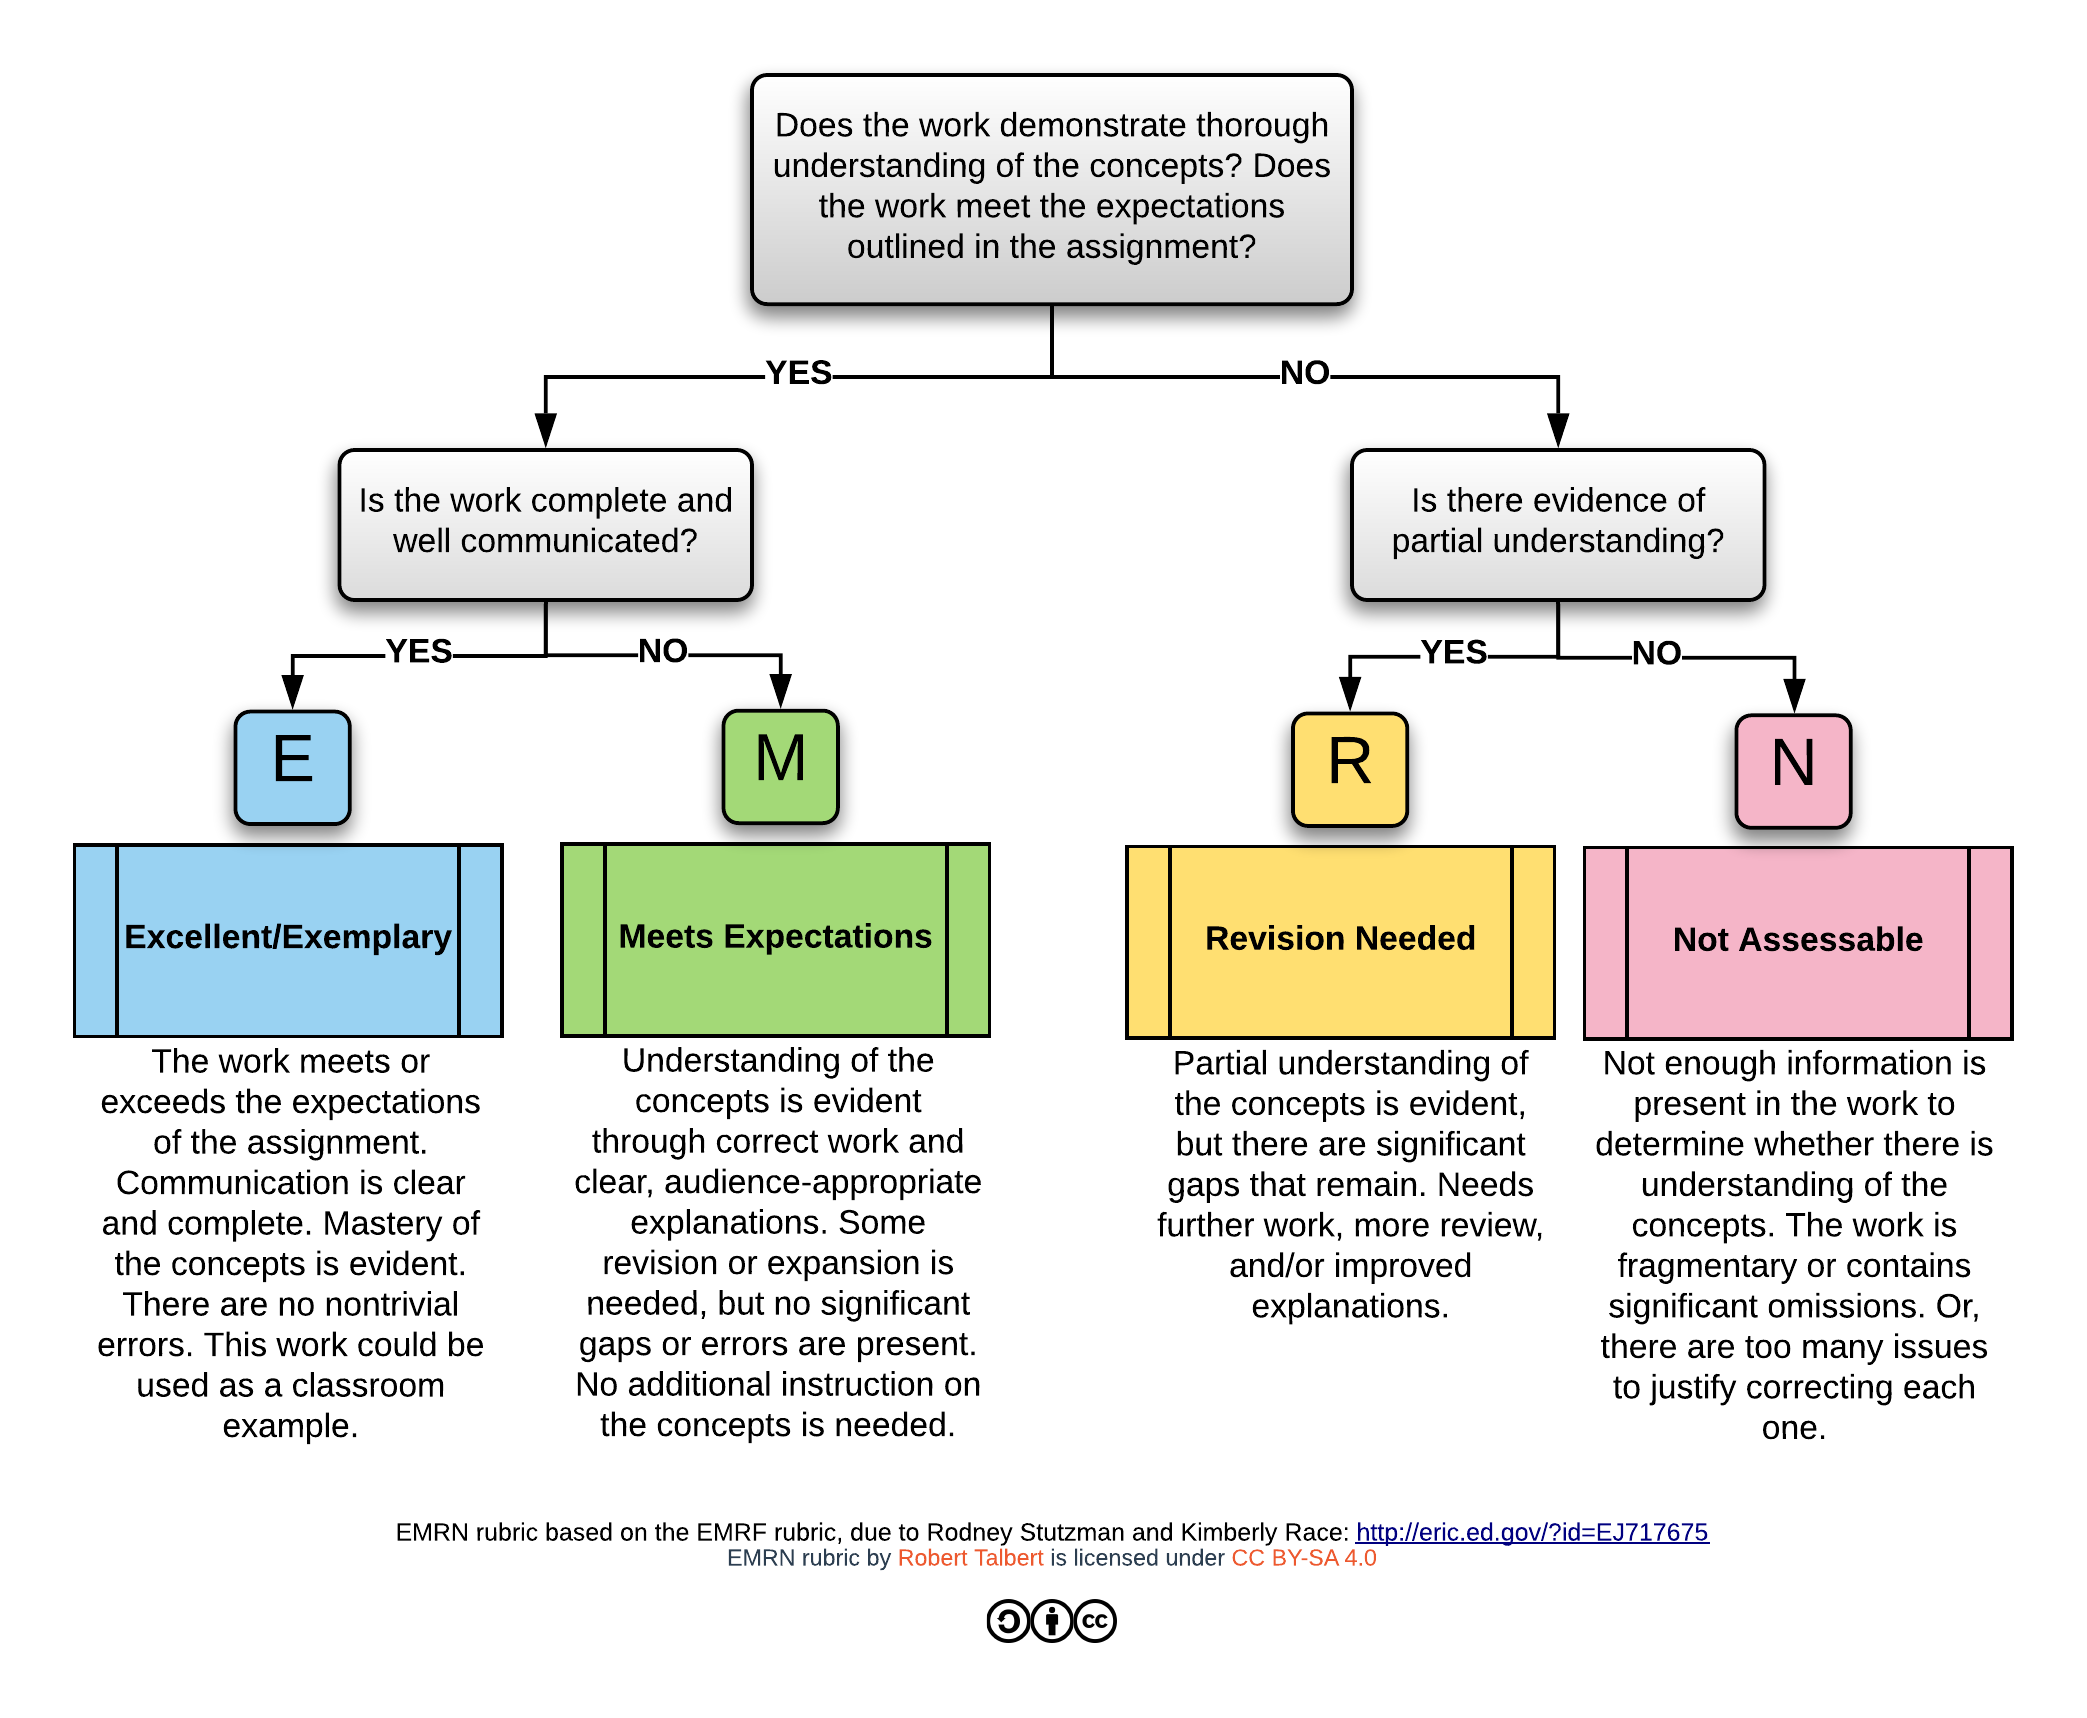
\includegraphics{EMRN-rubric-2020.png}
\caption{EMRN rubric}
\end{figure}

Each lab report can be revised and resubmitted before the grade becomes
final. Deadlines and conditions for submission of revised reports will
be communicated in Canvas.

\begin{itemize}
\tightlist
\item
  Grade ``E'' or ``M'' receives full score (5\%)
\item
  Grade ``R'' will receive partial score (3\%) with an option to revise
  and resubmit.
\item
  Grade ``N'' will receive partial score (2\%) with an option to revise
  and resubmit but the feedback will be very limited.
\item
  No report will not receive credit (0\%). Submissions after the
  deadline will be reviewed as-is with no possibility for revision and
  resubmission.
\end{itemize}

\subsubsection{Research report and
presentation}\label{research-report-and-presentation}

Written reports and oral presentations will be evaluated using the
\href{https://drive.google.com/file/d/1ZAL5_sTpci3waFMQVWRrhFqTF9uOIwv9/view?usp=sharing}{ELIPSS
rubric}. Enhancing Learning by Improving Process Skills in STEM (ELIPSS)
is an NSF-funded project that focuses on the identification,
development, and assessment of process skills (also known as
professional skills, practical skills, workplace skills, transferable
skills, or soft skills) in active learning, undergraduate STEM
classrooms. Assessing process skill development and providing feedback
to students and instructors is a key component for enhancing these
skills in STEM programs.
